
%-------------------------------------------------------------------------------------
Los Ingenieros de la empresa le presentan el siguiente Anillo óptico DWDM como bosquejo de diseño para comunicar sus 4 principales centros de datos en Santiago con fibra monomodo de dispersión desplazada a 10Gbps y uso de $\lambda$ transporte en banda C con frecuencia central nominal a 193.2 Thz según norma ITU-T G.694.1:
\begin{figure}
	\centering
	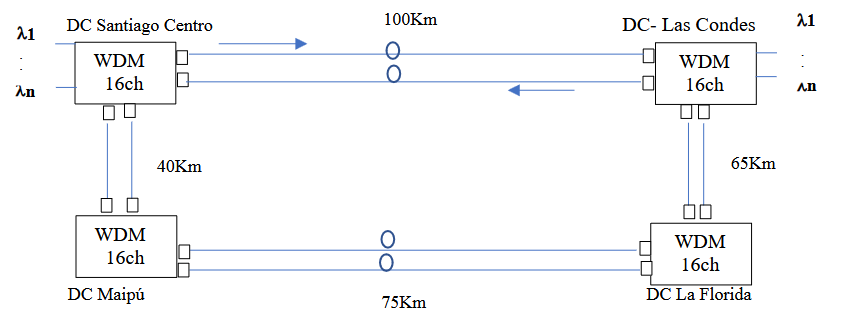
\includegraphics[width=0.7\linewidth]{img/ejemplos/Figure_1}
	\caption{Anillo Óptico DWDM}
	\label{fig:anillo}
\end{figure}
\begin{table}[h!]
	\centering
	\begin{tabular}{|l|l|}
	\hline
	\multicolumn{2}{|c|}{\textbf{Características Transponders Ópticos}} \\ \hline
	\textbf{Parámetro}                  & \textbf{Valor}                 \\ \hline
	Potencia de entrada                 & 2.3 dBm                        \\ \hline
	Sensibilidad óptica ($Se$)          & -30 dBm con BER $< 10^{-9}$    \\ \hline
	Potencia de saturación              & -10 dBm                        \\ \hline
	Margen de Seguridad                 & 1 dB                           \\ \hline
	Pérdida por conectores              & 0.5 dB                         \\ \hline
	Carretes de FO                      & 10 Km y 5 Km                   \\ \hline
	Pérdida por empalmes                & 0.03 dB                        \\ \hline
	Atenuación de la fibra              & 0.2 dB/Km                      \\ \hline
	\end{tabular}
	\end{table}
	
	\begin{table}[h!]
	\centering
	\begin{tabular}{|l|l|}
	\hline
	\multicolumn{2}{|c|}{\textbf{Datos de la Fibra}} \\ \hline
	\textbf{Parámetro}                         & \textbf{Valor}        \\ \hline
	Coeficiente Dispersión cromática total     & 0.05 ns/nm x Km @ 1550 nm \\ \hline
	Dispersión por Modo de Polarización        & 0.75 ps/Km$^2$        \\ \hline
	\end{tabular}
	\end{table}
	
	\begin{table}[h!]
	\centering
	\begin{tabular}{|l|l|}
	\hline
	\multicolumn{2}{|c|}{\textbf{Datos de la Fuente del Transponder}} \\ \hline
	\textbf{Parámetro}          & \textbf{Valor} \\ \hline
	Método de modulación        & NRZ            \\ \hline
	Anchura Espectral (W)       & 0.01 nm        \\ \hline
	Tiempo de Subida del generador & 2 ps          \\ \hline
	Tiempo de Subida del fotodetector & 1 ps       \\ \hline
	\end{tabular}
	\end{table}
\newpage
%--------------------------------------------------------------------------------------
\begin{itemize}
	\item \textbf{Calcular para cada tramo la Potencia de salida dBm utilizando la ecuación de Balance óptico y concluya o recomiende qué hacer en caso de que la potencia de salida no se encuentre 3 dB por arriba de la sensibilidad óptica del transponder ($P_s = S_e + 3 \, \text{dB}$).}\\\\
	Se busca obtener la potencia de salida en dBm para cada tramo del sistema óptico DWDM de 16 canales (con sólo 2 canales habilitados). Para esto, se hace uso de la ecuación de balance óptico. La potencia de salida debe ser 3 dB por arriba de la sensibilidad óptica del transponder, es decir, \(P_{\text{salida}} = S_e + 3 \, \text{dB}\). Si la potencia de salida no cumple con esta condición, se deben realizar ajustes en el sistema óptico para que la potencia de salida sea mayor a la sensibilidad óptica del transponder. La ecuación de balance óptico está dada por:
	\begin{align}
	P_{\text{salida}} = P_{\text{entrada}} - P_{\text{Pérdida total}}
	\end{align}
	Luego, se considerará una potencia de entrada de 2.3 dBm y se calcularán las pérdidas totales para cada tramo. Las pérdidas totales se calcularán como:
	\begin{align}
		P_{\text{totales}} = P_{\text{fibra}} + P_{\text{Conectores}} + P_{\text{Empalmes}}
	\end{align}
\begin{itemize}
    \item Pérdidas Totales = Pérdidas por fibra + Pérdidas por conectores + Pérdidas por empalmes.
\end{itemize}
Se calculan las pérdidas totales para cada tramo:

\begin{table}[H]
	\centering
	\renewcommand{\arraystretch}{1.5} % Espaciado entre filas
	\begin{tabular}{|l|c|}
	\hline
	\multicolumn{2}{|c|}{\textbf{Tramo 1: DC Santiago Centro a DC Las Condes (100 Km)}} \\ \hline
	Pérdidas por fibra                 & $0.2 \, \text{dB/km} \times 100 \, \text{km} = 20 \, \text{dB}$ \\ \hline
	Pérdidas por conectores (2)        & $0.5 \, \text{dB} \times 2 = 1 \, \text{dB}$                    \\ \hline
	Pérdidas por empalmes (9)          & $0.03 \, \text{dB} \times 9 = 0.27 \, \text{dB}$                \\ \hline
	Margen de seguridad                & $1 \, \text{dB}$                                               \\ \hline
	\end{tabular}
	\caption{Cálculos de pérdidas para el Tramo 1: Santiago Centro - Las Condes (100 Km).}
	\label{tabla:tramo1}
\end{table}
Luego, el cálculo estará dado por:
\begin{align}
\text{Pérdidas totales} &= 20 + 1 + 0.27 + 1 = 22.27 \, \text{dB}, \\
\text{Potencia de salida} &= 2.3 \, \text{dBm} - 22.27 \, \text{dB} = -19.97 \, \text{dBm}, \\
\text{Potencia esperada} &= -30 \, \text{dBm} + 3 \, \text{dB} = -27 \, \text{dBm}.
\end{align}
Por lo tanto, la potencia de salida de \(-19.97 \, \text{dBm}\) está por encima de \(-27 \, \text{dBm}\), por lo que no se necesita ningún ajuste en este tramo.

\begin{table}[H]
	\centering
	\renewcommand{\arraystretch}{1.5} % Espaciado entre filas
	\begin{tabular}{|l|c|}
	\hline
	\multicolumn{2}{|c|}{\textbf{Tramo 2: Santiago Centro - Maipú (40 Km)}} \\ \hline
	\textbf{Concepto}               & \textbf{Cálculo}                               \\ \hline
	Atenuación por fibra            & $0.2 \, \text{dB/km} \times 40 \, \text{km} = 8 \, \text{dB}$ \\ \hline
	Pérdidas por conectores (2)     & $0.5 \, \text{dB} \times 2 = 1 \, \text{dB}$    \\ \hline
	Pérdidas por empalmes (3)       & $0.03 \, \text{dB} \times 3 = 0.09 \, \text{dB}$ \\ \hline
	Margen de seguridad             & $1 \, \text{dB}$                               \\ \hline
	\end{tabular}
	\caption{Cálculos de pérdidas para el Tramo 2: Santiago Centro - Maipú (40 Km).}
	\label{tabla:tramo2}
\end{table}
Luego, se tiene que la potencia será:
\begin{align}
\text{Atenuación total} &= 8 + 1 + 0.09 + 1 = 10.09 \, \text{dB}, \\
\text{Potencia de salida} &= 2.3 \, \text{dBm} - 10.09 \, \text{dB} = -7.79 \, \text{dBm}, \\
\text{Potencia esperada} &= -30 \, \text{dBm} + 3 \, \text{dB} = -27 \, \text{dBm}.
\end{align}
Por lo tanto, la potencia de salida de \(-7.79 \, \text{dBm}\) está por encima de \(-27 \, \text{dBm}\), por lo que no se necesita ningún ajuste en este tramo.

\begin{table}[H]
	\centering
	\renewcommand{\arraystretch}{1.5} % Espaciado entre filas
	\begin{tabular}{|l|c|}
	\hline
	\multicolumn{2}{|c|}{\textbf{Tramo 3: DC Maipú - DC La Florida (75 Km)}} \\ \hline
	Atenuación por fibra            & $0.2 \, \text{dB/km} \times 75 \, \text{km} = 15 \, \text{dB}$ \\ \hline
	Pérdidas por conectores (2)     & $0.5 \, \text{dB} \times 2 = 1 \, \text{dB}$                    \\ \hline
	Pérdidas por empalmes (7)       & $0.03 \, \text{dB} \times 7 = 0.21 \, \text{dB}$                \\ \hline
	Margen de seguridad             & $1 \, \text{dB}$                                               \\ \hline
	\end{tabular}
	\caption{Cálculos de pérdidas para el Tramo 3: DC Maipú - DC La Florida (75 Km).}
	\label{tabla:tramo3}
\end{table}
Luego, se tiene que la potencia será:
\begin{align}
\text{Atenuación total} &= 15 + 1 + 0.21 + 1 = 17.21 \, \text{dB}, \\
\text{Potencia de salida} &= 2.3 \, \text{dBm} - 17.21 \, \text{dB} = -14.91 \, \text{dBm}, \\
\text{Potencia esperada} &= -30 \, \text{dBm} + 3 \, \text{dB} = -27 \, \text{dBm}.
\end{align}
Por lo tanto, la potencia de salida de \(-14.91 \, \text{dBm}\) está por encima de \(-27 \, \text{dBm}\), por lo que no se necesita ningún ajuste en este tramo.

\begin{table}[H]
	\centering
	\renewcommand{\arraystretch}{1.5} % Espaciado entre filas
	\begin{tabular}{|l|c|}
	\hline
	\multicolumn{2}{|c|}{\textbf{Tramo 4: DC Las Condes - DC La Florida (65 Km)}} \\ \hline
	Atenuación por fibra            & $0.2 \, \text{dB/km} \times 65 \, \text{km} = 13 \, \text{dB}$ \\ \hline
	Pérdidas por conectores (2)     & $0.5 \, \text{dB} \times 2 = 1 \, \text{dB}$                    \\ \hline
	Pérdidas por empalmes (6)       & $0.03 \, \text{dB} \times 6 = 0.18 \, \text{dB}$                \\ \hline
	Margen de seguridad             & $1 \, \text{dB}$                                               \\ \hline
	\end{tabular}
	\caption{Cálculos de pérdidas para el Tramo 4: DC Las Condes - DC La Florida (65 Km).}
	\label{tabla:tramo4}
\end{table}
Luego, se tiene que la potencia será:
\begin{align}
\text{Atenuación total} &= 13 + 1 + 0.18 + 1 = 15.18 \, \text{dB}, \\
\text{Potencia de salida} &= 2.3 \, \text{dBm} - 15.18 \, \text{dB} = -12.88 \, \text{dBm}, \\
\text{Potencia esperada} &= -30 \, \text{dBm} + 3 \, \text{dB} = -27 \, \text{dBm}.
\end{align}
Por lo tanto, la potencia de salida de \(-12.88 \, \text{dBm}\) está por encima de \(-27 \, \text{dBm}\), por lo que no se necesita ningún ajuste en este tramo.

En todos los tramos, la potencia de salida es suficientemente alta y se encuentra dentro del rango aceptable, ya que siempre es superior a \(-27 \, \text{dBm}\). Por lo tanto, no es necesario realizar ajustes ni agregar atenuadores ópticos.


%-------------------------------------------------------------------------------------
\item \textbf{Indicar en qué tramo agregaría un Atenuador óptico del tipo FOA, describa para qué sirve y su valor de atenuación recomendado}\\\\
En base a los cálculos realizados para el ítem 1.a, la potencia de salida en cada tramo se mantiene por encima de la sensibilidad óptica del transponder (diferencia de al menos 3 dB), lo que significa que no se requiere la adición de un atenuador óptico (FOA) en ninguno de los tramos para mantener una señal adecuada.\\\\
Un Atenuador Óptico FOA (Fiber Optic Attenuator) es un dispositivo utilizado en sistemas de comunicaciones ópticas para reducir la potencia de la señal óptica sin distorsionar la información transmitida. Su principal función es ajustar la potencia de la señal a niveles apropiados para evitar que el receptor, como un transponder o fotodetector, se sature debido a una señal demasiado fuerte. Esto es especialmente importante en enlaces ópticos de larga distancia o cuando se conectan diferentes segmentos de fibra que pueden generar potencias desiguales. Un atenuador óptico asegura que la potencia de la señal no exceda los límites operativos del equipo receptor.\\\\
El atenuador óptico FOA también se utiliza para garantizar un rendimiento óptimo de la red, manteniendo la señal en un rango ideal para la transmisión sin pérdidas ni interferencias. Existen atenuadores fijos, que proporcionan un nivel constante de atenuación, y variables, que permiten ajustar la atenuación según las necesidades específicas de la red. En general, su uso es fundamental para mantener la integridad de la señal óptica, evitar la saturación del equipo y optimizar la calidad de la comunicación en una red de fibra óptica.\\\\
No se requieren atenuadores ópticos en los tramos analizados, ya que los niveles de potencia de salida están suficientemente dentro de los límites operativos del transponder. Por lo tanto, no se recomienda agregar un atenuador óptico FOA en ningún tramo.\\\\
Si hubiera sido necesario, el valor de atenuación recomendado sería aquel que reduzca la potencia de salida para que esté 1 dB por encima de la sensibilidad óptica del transponder ($P_{\text{out}} > P_{\text{sens}} + 3 \, \text{dB}$), pero en este caso no se requiere.
%-------------------------------------------------------------------------------------
\item \textbf{Calcular para cada tramo los Tiempos de Procesamiento de Subida de la FO y Equipo, y concluya o recomiende qué hacer en caso de que no se cumpla que el Tiempo de Subida de la FO sea menor al Tiempo de Subida del Equipo, y recomiende qué modificaciones haría en el diseño en caso de que algún tramo no se cumpla la condición.}\\\\
Se busca obtener el tiempo de procesamiento de subida de la fibra óptica y del equipo para cada tramo del sistema óptico DWDM de 16 canales (con sólo 2 canales habilitados). Para esto, se hace uso de los datos proporcionados en el enunciado. Se debe cumplir que el tiempo de subida de la fibra óptica sea menor al tiempo de subida del equipo, de lo contrario se deben realizar ajustes en el diseño para que se cumpla esta condición.

\begin{itemize}
	\item \textbf{Dispersión Cromática Total (\(T_{\text{crom}}\)):} La dispersión cromática total (\(T_{\text{crom}}\)) se calcula sumando los coeficientes de dispersión cromática material y guía de onda, multiplicados por la anchura espectral del generador óptico y la longitud del enlace.
	\begin{align}
	T_{\text{crom}} &= (D_{\text{rommat}} + D_{\text{romguía}}) \times W_{\text{spectral}} \times L
	\end{align}
	\item \textbf{Dispersión Total (\(T_{\text{FO}}\)):} La dispersión total (\(T_{\text{FO}}\)) se obtiene combinando la dispersión cromática total y la dispersión por modo de polarización (PMD) utilizando la fórmula:
	\begin{align}
	T_{\text{FO}} &= \sqrt{T_{\text{crom}}^2 + T_{\text{PMD}}^2}
	\end{align}
	\item \textbf{Dispersión por Modo de Polarización (PMD):} 
	\begin{align}
	T_{\text{PMD}} &= \text{PMD} \times \sqrt{L}
	\end{align}
	\item \textbf{Tiempos de Subida del Equipo (\(T_{\text{Equipo}}\)):} 
	El tiempo de subida del equipo (\(T_{\text{Equipo}}\)) se calcula restando los tiempos de subida del generador (\(T_{\text{gen}}\)) y del fotodetector (\(T_{\text{rx}}\)) del tiempo de subida total del sistema (\(T_{\text{sist}}\)).
	\begin{align}
	T_{\text{Equipo}} &= \sqrt{T_{\text{sist}}^2 - T_{\text{gen}}^2 - T_{\text{rx}}^2}
	\end{align}
	El tiempo de subida total del sistema (\(T_{\text{sist}}\)) se calcula utilizando el ancho de banda eléctrico del sistema (\(B_{\text{sist.Eléctrico}}\)) como:
	\begin{align}
	B_{\text{sist.Eléctrico}} &= \frac{R_{\text{NRZ}}}{2} \\
	B_{\text{sist.Eléctrico}} &= \frac{10}{2} = 5 \, \text{GHz}
	\end{align}
	Por lo tanto, el \(T_{\text{sist}}\) es:
	\begin{align}
	T_{\text{sist}} &= \frac{0.35}{B_{\text{sist.Eléctrico}}} \\
	T_{\text{sist}} &= \frac{0.35}{5} = 0.07 \, \text{ns} = 70 \, \text{ps}
	\end{align}
	Finalmente, el tiempo de subida del equipo (\(T_{\text{Equipo}}\)) se determina como:
	\begin{align}
	T_{\text{Equipo}} &= \sqrt{T_{\text{sist}}^2 - T_{\text{gen}}^2 - T_{\text{rx}}^2} \\
	T_{\text{Equipo}} &= \sqrt{70^2 - 2^2 - 1^2} = 69.96 \, \text{ps}
	\end{align}
\end{itemize}

\begin{table}[H]
	\centering
	\renewcommand{\arraystretch}{1.5}
	\begin{tabular}{|l|c|}
		\hline
		\multicolumn{2}{|c|}{\textbf{Tramo 1: DC Santiago Centro a DC Las Condes (100 Km)}} \\ \hline
		Dispersión cromática                      & $0.05 \, \text{ns/nm km} \times 0.01 \, \text{nm} \times 100 \, \text{km} = 50 \, \text{ps}$ \\ \hline
		Dispersión por modo de polarización (TPMD) & $0.75 \, \text{ps/km} \times \sqrt{2 \times 100} = 7.5 \, \text{ps}$ \\ \hline
		Dispersión total en la FO (\(T_{\text{FO}}\)) & $\sqrt{50^2 + 7.5^2} = 50.56 \, \text{ps}$ \\ \hline
	\end{tabular}
	\caption{Cálculos resumidos para el Tramo 1.}
\end{table}

Por lo tanto, el tiempo de subida de la FO (50.56 ps) es menor que el tiempo de subida del equipo (69.96 ps), por lo que este tramo cumple con la condición y no requiere modificación.

\begin{table}[H]
	\centering
	\renewcommand{\arraystretch}{1.5}
	\begin{tabular}{|l|c|}
		\hline
		\multicolumn{2}{|c|}{\textbf{Tramo 2: DC Santiago Centro a DC Maipú (40 Km)}} \\ \hline
		Dispersión cromática                      & $0.05 \, \text{ns/nm km} \times 0.01 \, \text{nm} \times 40 \, \text{km} = 20 \, \text{ps}$ \\ \hline
		Dispersión por modo de polarización (TPMD) & $0.75 \, \text{ps/km} \times \sqrt{2 \times 40} = 4.74 \, \text{ps}$ \\ \hline
		Dispersión total en la FO (\(T_{\text{FO}}\)) & $\sqrt{20^2 + 4.74^2} = 20.55 \, \text{ps}$ \\ \hline
	\end{tabular}
	\caption{Cálculos resumidos para el Tramo 2.}
\end{table}

Por lo tanto, el tiempo de subida de la FO (20.55 ps) es menor que el tiempo de subida del equipo (69.96 ps), por lo que este tramo cumple con la condición y no requiere modificación.

\begin{table}[H]
	\centering
	\renewcommand{\arraystretch}{1.5}
	\begin{tabular}{|l|c|}
		\hline
		\multicolumn{2}{|c|}{\textbf{Tramo 3: DC Maipú a DC La Florida (75 Km)}} \\ \hline
		Dispersión cromática                      & $0.05 \, \text{ns/nm km} \times 0.01 \, \text{nm} \times 75 \, \text{km} = 37.5 \, \text{ps}$ \\ \hline
		Dispersión por modo de polarización (TPMD) & $0.75 \, \text{ps/km} \times \sqrt{2 \times 75} = 6.5 \, \text{ps}$ \\ \hline
		Dispersión total en la FO (\(T_{\text{FO}}\)) & $\sqrt{37.5^2 + 6.5^2} = 38.06 \, \text{ps}$ \\ \hline
	\end{tabular}
	\caption{Cálculos resumidos para el Tramo 3.}
\end{table}

Por lo tanto, el tiempo de subida de la FO (38.06 ps) es menor que el tiempo de subida del equipo (69.96 ps), por lo que este tramo cumple con la condición y no requiere modificación.

\begin{table}[H]
	\centering
	\renewcommand{\arraystretch}{1.5}
	\begin{tabular}{|l|c|}
		\hline
		\multicolumn{2}{|c|}{\textbf{Tramo 4: DC Las Condes a DC La Florida (65 Km)}} \\ \hline
		Dispersión cromática                      & $0.05 \, \text{ns/nm km} \times 0.01 \, \text{nm} \times 65 \, \text{km} = 32.5 \, \text{ps}$ \\ \hline
		Dispersión por modo de polarización (TPMD) & $0.75 \, \text{ps/km} \times \sqrt{2 \times 65} = 6.05 \, \text{ps}$ \\ \hline
		Dispersión total en la FO (\(T_{\text{FO}}\)) & $\sqrt{32.5^2 + 6.05^2} = 33.06 \, \text{ps}$ \\ \hline
	\end{tabular}
	\caption{Cálculos resumidos para el Tramo 4.}
\end{table}

Por lo tanto, el tiempo de subida de la FO (33.06 ps) es menor que el tiempo de subida del equipo (69.96 ps), por lo que este tramo cumple con la condición y no requiere modificación.

	%-------------------------------------------------------------------------------------
	\item \textbf{Utilizando el Simulador OptiSystem diseñe para cada uno de los tramos el
	sistema óptico DWDM de 16ch (con sólo 2 canales habilitados) por cada tramo
	incluyendo las recomendaciones realizadas en el punto anterior 1a y 1b, si ameritan,
	para presentar al CEO, que permita validar los parámetros ópticos entregados.
	Presentar:}
	\item Captura de Pantalla de Diseño óptico global en OptiSystem, capturas de pantalla de los parámetros configurados por cada componente y uso de herramientas de visualización para ver las potencias ópticas y pérdidas del sistema.\\\\
Se busca diseñar los tramos del sistema óptico DWDM de 16 canales (con sólo 2 canales habilitados). Para esto, se utiliza la herramienta OptiSystem, donde se configuran los parámetros de cada componente y se visualizan las potencias ópticas y pérdidas del sistema.

\begin{figure}[H]
	\centering
	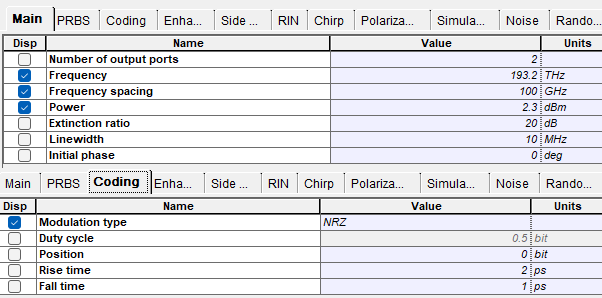
\includegraphics[width=0.8\linewidth]{img/ejemplos/Figure_2}
	\caption{Configuración para el transmisor en relación con los parámetros entregados.}
	\label{fig:optisystem_tx}
\end{figure}

\begin{figure}[H]
	\centering
	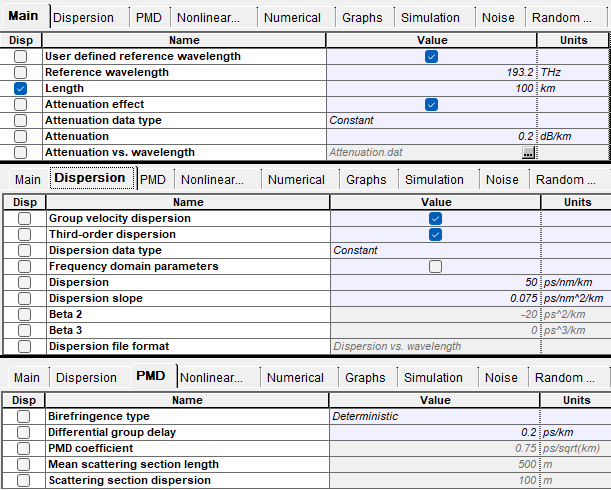
\includegraphics[width=0.7\linewidth]{img/ejemplos/Figure_3}
	\caption{Configuración para la fibra óptica en relación con los parámetros entregados.}
	\label{fig:optisystem_fiber}
\end{figure}

El esquema global para cada tramo se presenta a continuación:

\begin{figure}[H]
	\centering
	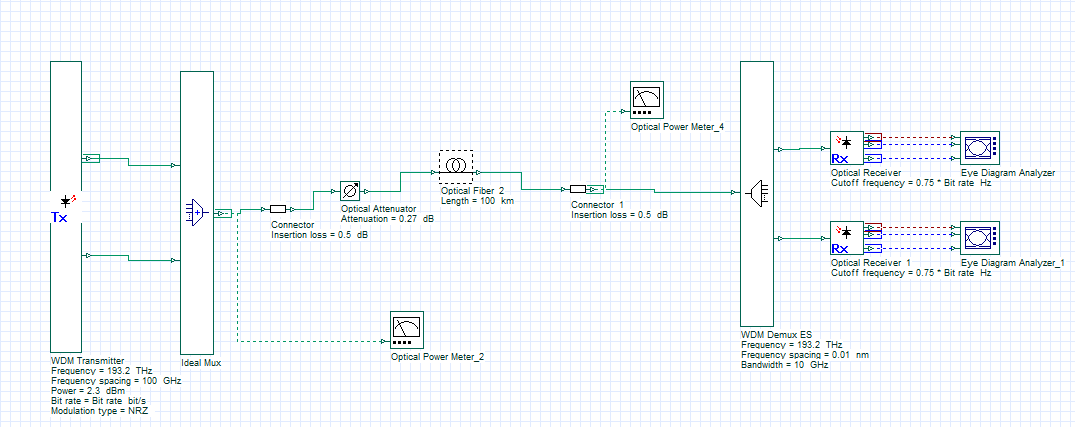
\includegraphics[width=0.9\linewidth]{img/ejemplos/Figure_4}
	\caption{Esquema global del sistema óptico DWDM para el Tramo 1.}
	\label{fig:optisystem_tramo1}
\end{figure}

\begin{figure}[H]
	\centering
	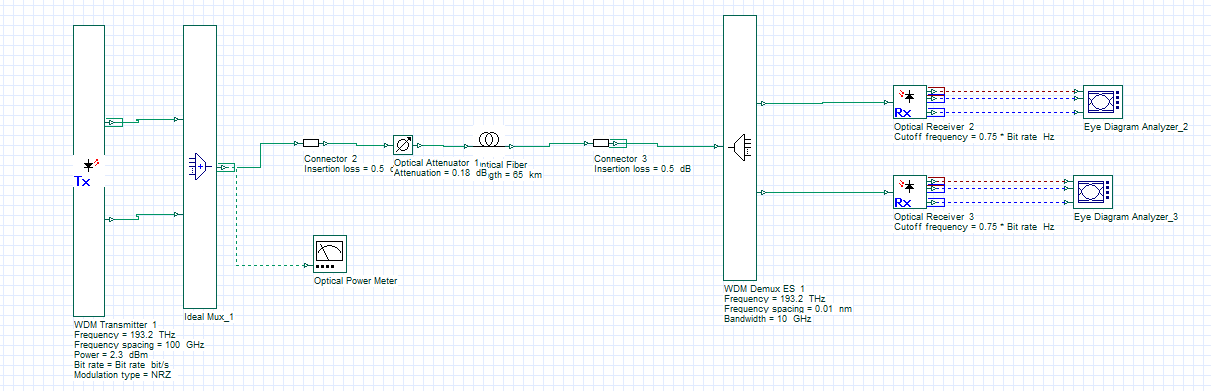
\includegraphics[width=0.9\linewidth]{img/ejemplos/Figure_5}
	\caption{Esquema global del sistema óptico DWDM para el Tramo 2.}
	\label{fig:optisystem_tramo2}
\end{figure}

\begin{figure}[H]
	\centering
	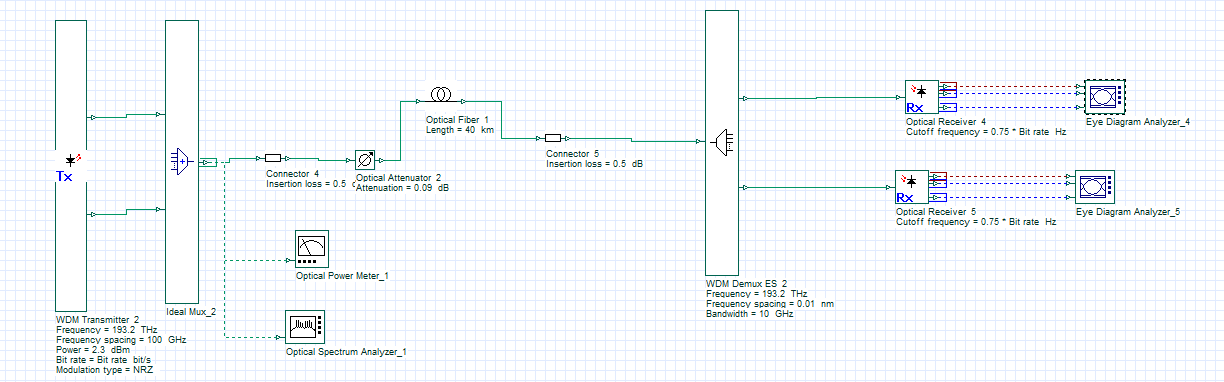
\includegraphics[width=0.9\linewidth]{img/ejemplos/Figure_6}
	\caption{Esquema global del sistema óptico DWDM para el Tramo 3.}
	\label{fig:optisystem_tramo3}
\end{figure}

\begin{figure}[H]
	\centering
	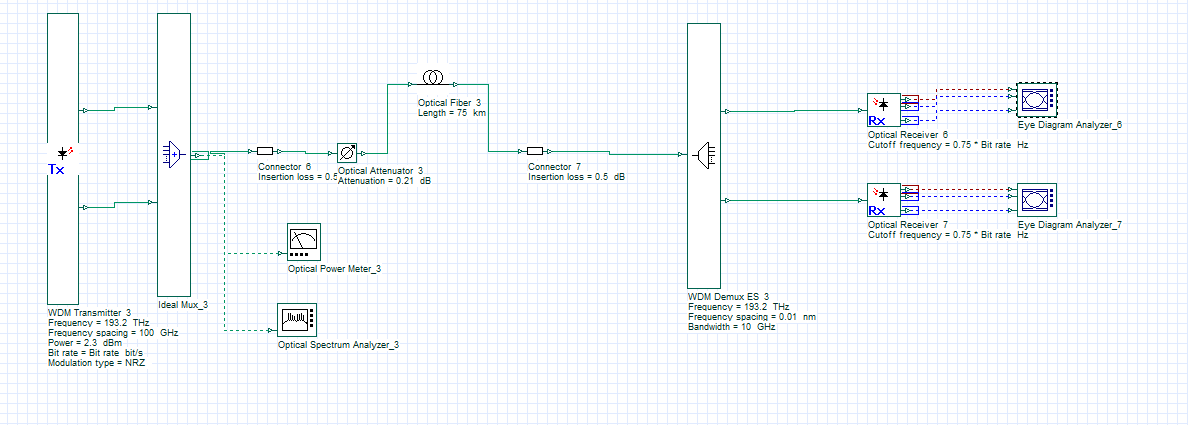
\includegraphics[width=0.9\linewidth]{img/ejemplos/Figure_7}
	\caption{Esquema global del sistema óptico DWDM para el Tramo 4.}
	\label{fig:optisystem_tramo4}
\end{figure}
%-------------------------------------------------------------------------------------
\item \textbf{Capturas de pantalla de Diagrama de Ojo. Compare las formas y analice el BER para cada tramo y concluya si es posible obtener el OSNR por tramo.}\\\\
Se obtienen los diferentes diagramas de ojo para los diferentes tramos, que se presentan a continuación:

\begin{figure}[H]
	\centering
	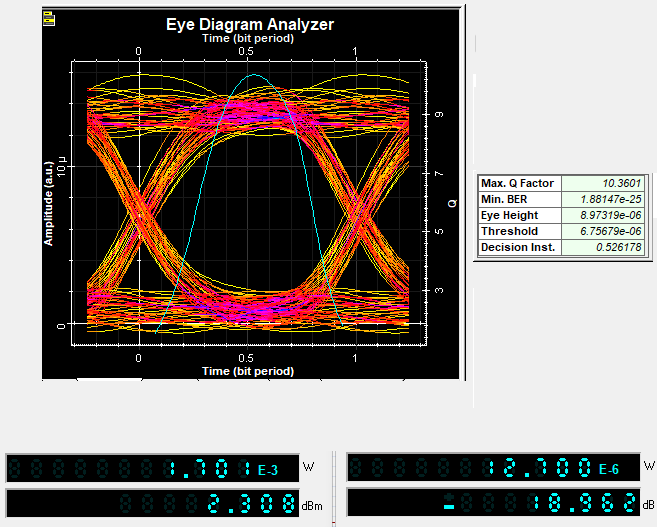
\includegraphics[width=0.6\linewidth]{img/ejemplos/Figure_8}
	\caption{Diagrama de Ojo para el Tramo 1, junto con la potencia de salida y la potencia recibida.}
	\label{fig:optisystem_eye1}
\end{figure}

\begin{figure}[H]
	\centering
	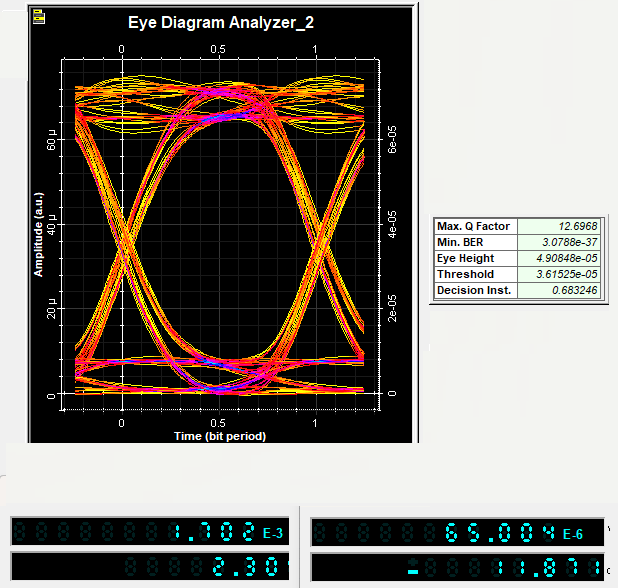
\includegraphics[width=0.6\linewidth]{img/ejemplos/Figure_9}
	\caption{Diagrama de Ojo para el Tramo 2, junto con la potencia de salida y la potencia recibida.}
	\label{fig:optisystem_eye2}
\end{figure}

\begin{figure}[H]
	\centering
	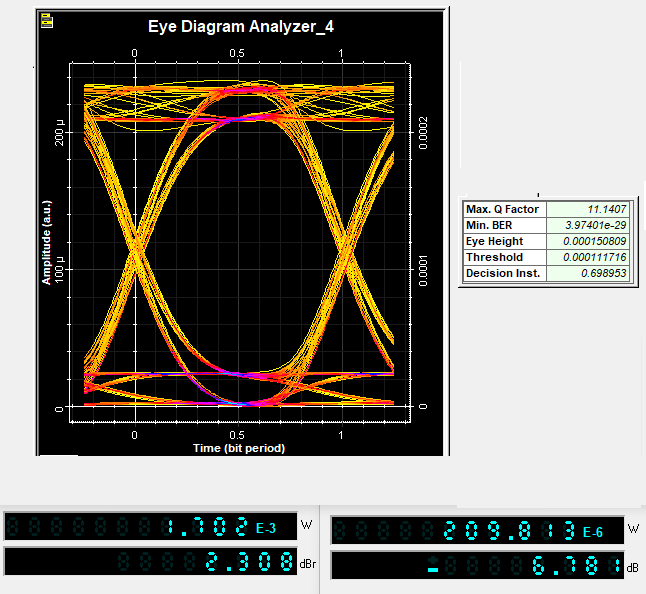
\includegraphics[width=0.6\linewidth]{img/ejemplos/Figure_10}
	\caption{Diagrama de Ojo para el Tramo 3, junto con la potencia de salida y la potencia recibida.}
	\label{fig:optisystem_eye3}
\end{figure}

\begin{figure}[H]
	\centering
	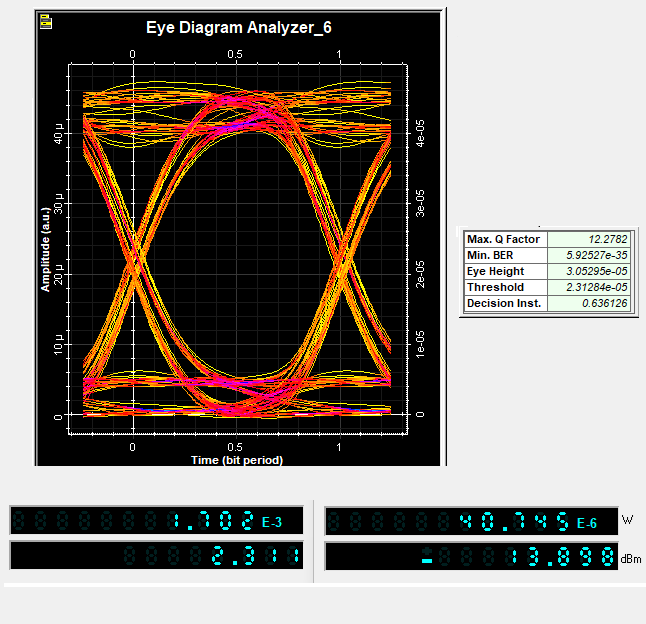
\includegraphics[width=0.6\linewidth]{img/ejemplos/Figure_11}
	\caption{Diagrama de Ojo para el Tramo 4, junto con la potencia de salida y la potencia recibida.}
	\label{fig:optisystem_eye4}
\end{figure}

La comparación de los diferentes diagramas de ojo para los tramos se muestra en la siguiente figura:

\begin{figure}[H]
	\centering
	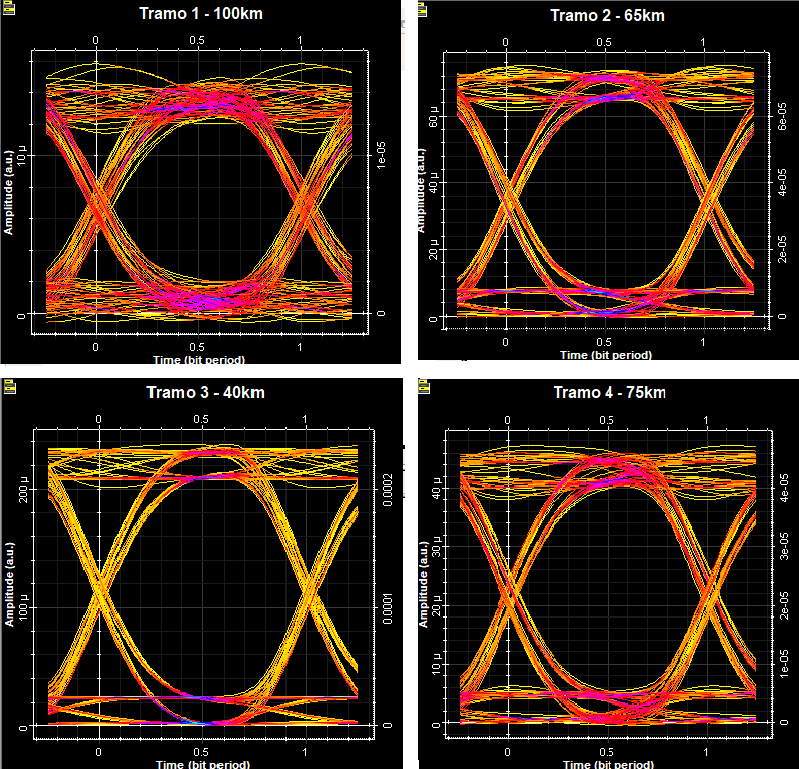
\includegraphics[width=0.6\linewidth]{img/ejemplos/Figure_12}
	\caption{Comparación de los Diagramas de Ojo para los 4 tramos del sistema óptico DWDM.}
	\label{fig:optisystem_eye_comparison}
\end{figure}
%-------------------------------------------------------------------------------------
\item \textbf{Plantee recomendaciones al diseño para mejorar la transmisión de señal óptica en cada tramo.}\\\\
Para mejorar la transmisión de la señal óptica en cada tramo del sistema DWDM, se recomienda implementar las siguientes acciones:

\begin{itemize}
	\item \textbf{Uso de amplificadores ópticos (EDFA):} Colocar preamplificadores y post-amplificadores estratégicamente para garantizar niveles óptimos de potencia en los tramos largos, minimizando la degradación de la señal.
	\item \textbf{Compensación de dispersión cromática:} Incorporar módulos de fibra compensadora de dispersión (DCF) en los enlaces de más de 40 km para corregir la acumulación de dispersión cromática, manteniendo la integridad de la señal.
	\item \textbf{Control de dispersión por modo de polarización (PMD):} Asegurar el uso de fibras de baja dispersión por modo de polarización y componentes ópticos de alta calidad para reducir este efecto.
	\item \textbf{Monitoreo constante de parámetros clave:} Implementar herramientas de supervisión para evaluar el OSNR (relación señal a ruido óptica) y el BER (tasa de error de bits) en tiempo real para detectar problemas potenciales.
\end{itemize}

Con estas medidas, se busca maximizar la eficiencia del sistema, reducir errores de transmisión y mantener una alta calidad de señal óptica en todo el anillo DWDM.

	\item \textbf{Dado que este proyecto es muy estratégico para el CEO de la compañía, se requiere que se analicen 3 alternativas de proyectos de inversión para el Anillo óptico proyectado. Por otro lado, se espera que con este Anillo óptico de Core Bancario el Banco aumente sus Ingresos anuales proyectados en un 1\% de los US\$150 millones obtenidos el año pasado.}
	%-------------------------------------------------------------------------------------
	\item Obtener el ROI (Return on Invertion) de cada proyecto y hacer una Evaluación de Proyectos simple para cada uno de ellos calculando los Ingresos Anuales - Egresos Operacionales para obtener un
	Flujo de Caja del proyecto, que permitirá justificar económicamente el mejor proyecto de inversión según los indicadores económicos de cada proyecto: VAN, TIR y Payback en un horizonte de 3 años
	y una tasa de interés de costo de oportunidad del 10\% anual. Concluya desde un punto de vista económico cuál proyecto de mayor a menor tiene mejores retornos al inversionista.\\\\
	Se buscan obtener diversas metricas para cada uno de los proyectos de inversion, comenzando con el Valor Actual Neto (VAN) el cual es una medida financiera que se utiliza para evaluar la viabilidad de una inversión o proyecto. Se calcula sumando los valores presentes de todos los flujos de caja esperados de la inversión, descontados a una tasa de interés específica  (en este caso, el 10\% anual), y restando la inversión inicial.
	\begin{align}
		VAN &= \sum_{t=0}^{n} \frac{F_t}{(1+r)^t} - I
	\end{align}
	Donde:
	\begin{itemize}
    	\item $F_t$ es el flujo de caja en el período $t$.
    	\item $r$ es la tasa de descuento (10\% anual en este caso).
    	\item $t$ es el período de tiempo.
    	\item $I$ es la inversión inicial.
	\end{itemize}
	El VAN tiene una importante interpretacion la cual viene dada por:
	\begin{itemize}
    	\item \textbf{VAN es positivo}: la inversión es viable ya que generará más valor que el costo del capital.
	    \item \textbf{VAN es negativo}: la inversión no es viable ya que no cubrirá el costo del capital.
	\end{itemize}
	La Tasa Interna de Retorno (TIR) es la tasa de descuento que hace que el VAN sea igual a cero.Es una medida de la rentabilidad de una inversión. Básicamente, es la tasa de interés a la cual los flujos de caja descontados son iguales a la inversión inicial.
	\begin{align}
		VAN &= \sum_{t=0}^{n} \frac{F_t}{(1+\text{TIR})^t} - I = 0
	\end{align}
	La interpretacion que se tiene del TIR corresponde a lo siguiente:
	\begin{itemize}
    	\item \textbf{TIR es mayor:} que la tasa de descuento (costo de oportunidad del capital), la inversión es viable.
	    \item \textbf{TIR es menor:} que la tasa de descuento, la inversión no es viable.
	\end{itemize}
	Se tiene ademas que el periodo de Payback es el tiempo que tarda una inversión en recuperar su costo inicial a través de los flujos de caja netos que genera.  No tiene en cuenta el valor temporal del dinero, lo cual es una limitación importante. Este se logra interpretar como que un Un periodo de \textit{Payback} más corto es generalmente preferible ya que indica un menor tiempo de recuperación de la inversión. Por otro lado se tiene que el Retorno sobre la Inversión (ROI) es una medida de rendimiento utilizada para evaluar la eficiencia de una inversión. El ROI se calcula dividiendo el beneficio neto de la inversión por el costo de la inversión.
	\begin{align}
		ROI &= \frac{\text{Beneficio Neto}}{\text{Costo de Inversión}}
	\end{align}
	La interpretacion de este parametro viene dada por 
	\begin{itemize}
    	\item \textbf{ROI positivo:} indica que los beneficios de la inversión superan los costos, lo que representa una buena inversión.
    	\item \textbf{ROI negativo:} indica que los costos superan los beneficios, lo que representa una mala inversión.
    	\item \textbf{ROI alto:} es preferible, ya que indica una mayor eficiencia y rentabilidad de la inversión.
	\end{itemize}
	Se procedera a analizar los diferentes proyectos de inversion en base a los parametros anteriormente vistos:

	\begin{itemize}
		\item \textbf{Proyecto de Inversión 1:} Se puede observar que este proyecto de inversión muestra un VAN de \$2,175,098, lo que significa que genera valor presente significativo sobre el costo de capital. Además, su TIR es de 86.98\%, muy superior a la tasa de descuento del 10\%, indicando una rentabilidad altamente atractiva. El Payback es de solo 1 año, lo que implica un periodo de recuperación extremadamente rápido. Por último, el ROI del 50\% confirma que el retorno sobre la inversión inicial es positivo y competitivo.
	\begin{figure}
		\centering
		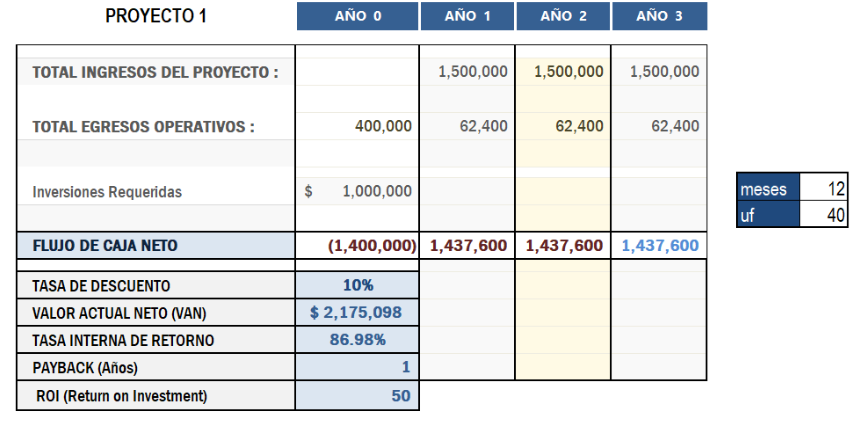
\includegraphics[width=0.9\linewidth]{img/ejemplos/Figure_13}
		\caption{Flujo de caja para el Proyecto de Inversión 1.}
		\label{fig:optisystem}
	\end{figure}
	\item \textbf{Proyecto de Inversión 2:} Esta propuesta muestra un VAN de \$1,031,856, indicando que genera valor adicional con una rentabilidad atractiva gracias a su TIR del 33.13\%, que supera ampliamente la tasa de descuento del 10\%. El periodo de recuperación (Payback) es de 1.27 años, destacando su rápido retorno. Sin embargo, el ROI de -14.3\% señala que la relación entre los beneficios generados y la inversión inicial no es favorable, probablemente debido al alto costo de implementación. A pesar de esto, los indicadores reflejan que el proyecto es económicamente viable.
	\begin{figure}
		\centering
		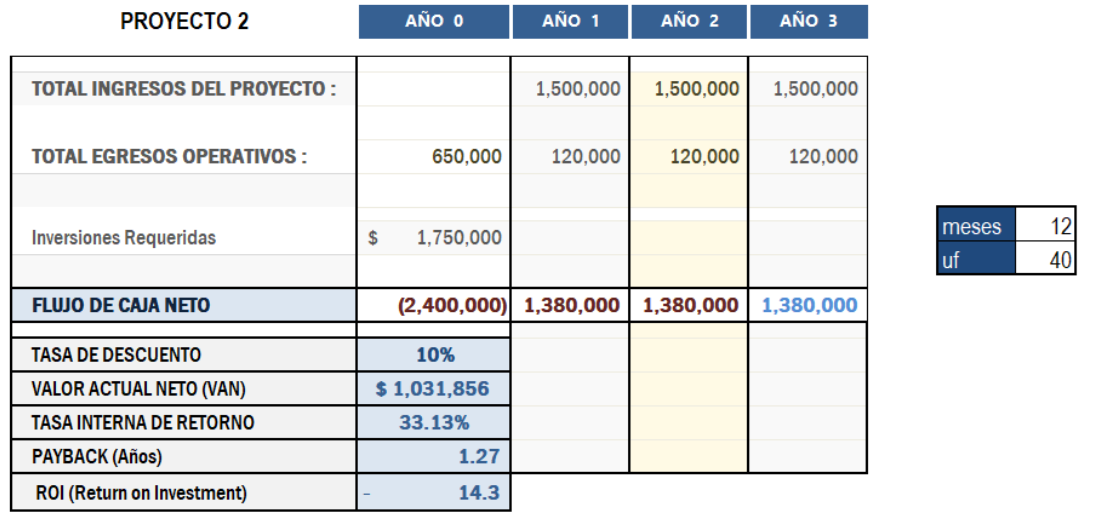
\includegraphics[width=0.9\linewidth]{img/ejemplos/Figure_14}
		\caption{Flujo de caja para el Proyecto de Inversión 2.}
		\label{fig:optisystem}
	\end{figure}
	\item \textbf{Proyecto de Inversión 3:}Esta propuesta presenta excelentes indicadores económicos. Su VAN de \$2,708,657 muestra un valor significativamente positivo, mientras que su \textbf{TIR de 144.23\%} refleja una rentabilidad muy superior a la tasa de descuento del 10\%. Además, el periodo de recuperación (Payback) es de solo 0.5 años, lo que resalta su rápido retorno de la inversión. El ROI de 114\% indica una alta relación entre los beneficios generados y la inversión inicial, consolidando al proyecto como altamente rentable y eficiente.
	\begin{figure}
		\centering
		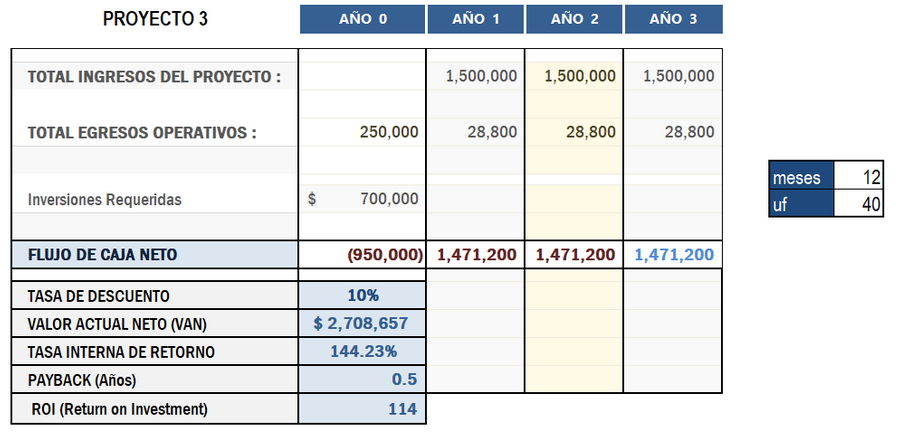
\includegraphics[width=0.9\linewidth]{img/ejemplos/Figure_15}
		\caption{Flujo de caja para el Proyecto de Inversión 3.}
		\label{fig:optisystem}
	\end{figure}
	\end{itemize}
	En conclusión, desde un punto de vista económico, el Proyecto 3 es el más rentable, destacando con un VAN de \$2,708,657, una TIR de 144.23\%, y un Payback de 0.5 años, lo que lo hace el de mayor retorno y el de recuperación más rápida. Le sigue el Proyecto 1, con un VAN de \$2,175,098, una TIR de 86.98\%, y un Payback de 1 año, siendo una opción sólida, aunque con un retorno más lento que el Proyecto 3. Finalmente, el Proyecto 2 presenta un VAN de \$1,031,856, una TIR de 33.13\%, y un Payback de 1.27 años, con un ROI negativo (-14.3\%), lo que lo hace menos atractivo comparado con los otros dos proyectos.
	%-------------------------------------------------------------------------------------
	\item Compare técnicamente para el proyecto de Anillo óptico las diferentes 3 tecnologías: DWDM
	OADM, DWDM ROADM y CWDM (explique cada una de ellas y compare técnicamente), y entregue su recomendación sólo desde un punto de vista técnico por capacidad y escalabilidad, cuál recomendaría:

	Se busca el evaluar las tecnologías disponibles para el anillo óptico, se analizarán las siguientes opciones: DWDM OADM, DWDM ROADMs y CWDM. El análisis se basa en los criterios de capacidad, escalabilidad, costo y aplicaciones prácticas. Comenzando con las caracteristicas  de DWDM OADM (Optical Add-Drop Multiplexer), se tiene lo siguiente:
	\begin{itemize}
   	 \item \textbf{Capacidad:} Utiliza múltiples longitudes de onda en la misma fibra óptica, con capacidad de agregar o eliminar ciertas longitudes de onda sin afectar las demás. Ofrece alta densidad espectral en la banda C (frecuencia central 193.1 THz).
   	 \item \textbf{Escalabilidad:} Limitada, ya que el número de longitudes de onda está fijo y las actualizaciones requieren intervención física.
   	 \item \textbf{Costo:} Moderado, más económico que los ROADMs, pero menos flexible.
   	 \item \textbf{Aplicaciones prácticas:} Ideal para implementaciones donde los nodos no requieren cambios dinámicos frecuentes y la configuración de tráfico es más estática.
	\end{itemize}
	Se tendra que sus ventajas seran:
	\begin{itemize}
    	\item Simplicidad en el diseño.
    	\item Costos moderados en comparación con los ROADMs.
    	\item Alta capacidad para conexiones de red estáticas.
	\end{itemize}
	Sus desventajas corresponderan a:
	\textbf{Desventajas:}
	\begin{itemize}
    	\item Escalabilidad limitada.
    	\item No permite reconfiguración automática de las rutas ópticas.
	\end{itemize}
	Luego tenemos la tecnología asociada a DWDM ROADMs (Reconfigurable Optical Add-Drop Multiplexer), la cual se caracteriza por:
	\begin{itemize}
    	\item \textbf{Capacidad:} Alta capacidad con múltiples longitudes de onda (típicamente 40, 80, o más canales DWDM). Permiten cambiar dinámicamente las rutas ópticas a través de la red.
    	\item \textbf{Escalabilidad:} Altamente escalable, con capacidad de modificar rutas y longitudes de onda remotamente sin intervención física.
    	\item \textbf{Costo:} Alto, debido a la complejidad del hardware y los sistemas de control.
    	\item \textbf{Aplicaciones prácticas:} Recomendado para redes donde se requiere alta flexibilidad, reconfiguración dinámica y optimización de rutas.
	\end{itemize}
	Se tendra que sus ventajas seran:	
	\begin{itemize}
    	\item Flexibilidad total en la gestión de rutas ópticas.
    	\item Escalabilidad dinámica sin necesidad de reconfiguración física.
    	\item Reducción de costos operativos a largo plazo en redes grandes y complejas.
	\end{itemize}
	Sus desventajas seran:	
	\begin{itemize}
    	\item Alto costo inicial.
    	\item Requiere una gestión más avanzada de la red.
	\end{itemize}
	Por ultimo se tiene la tecnologia asociada a CWDM (Coarse Wavelength Division Multiplexing), la cual se caracteriza por:
	\begin{itemize}
    	\item \textbf{Capacidad:} Capacidad limitada (generalmente 8 a 16 canales) en comparación con DWDM. Usa un espaciado más amplio entre longitudes de onda, lo que reduce la densidad espectral.
    	\item \textbf{Escalabilidad:} Moderada, adecuada para aplicaciones donde no se requiere una densidad espectral alta.
    	\item \textbf{Costo:} Bajo, ya que utiliza componentes ópticos más simples y menos precisos.
    	\item \textbf{Aplicaciones prácticas:} Mejor para redes de corta distancia y menores requisitos de capacidad.
	\end{itemize}
	Se tendra que sus ventajas seran:
	\begin{itemize}
    	\item Costo mucho más bajo en comparación con DWDM.
    	\item Menores requisitos técnicos en los transceptores ópticos.
    	\item Ideal para distancias cortas o aplicaciones donde no se necesita alta capacidad.
	\end{itemize}
	Sus desventajas seran:
	\begin{itemize}
    	\item Capacidad limitada.
    	\item No es adecuado para redes de largo alcance o de alta capacidad.
	\end{itemize}
	A continuación, se presenta una tabla resumen de las características principales de cada tecnología:
	\begin{center}
		\begin{tabular}{|l|c|c|c|}
		\hline
		\rowcolor[HTML]{D9E1F2} 
		\textbf{Criterio}            & \textbf{DWDM OADM} & \textbf{DWDM ROADMs} & \textbf{CWDM} \\ \hline
		\textbf{Capacidad}           & Alta               & Muy Alta             & Limitada      \\ \hline
		\textbf{Escalabilidad}       & Limitada           & Muy Alta             & Moderada      \\ \hline
		\textbf{Costo}               & Moderado           & Alto                 & Bajo          \\ \hline
		\textbf{Aplicaciones}        & Redes estáticas    & Redes dinámicas       & Redes cortas  \\ \hline
		\end{tabular}
	\end{center}
	Para este proyecto bancario, donde se priorizan la capacidad, escalabilidad y confiabilidad, se recomienda optar por \textbf{DWDM ROADMs}. Aunque el costo inicial es más alto, esta tecnología soporta configuraciones flexibles y una mayor densidad espectral, permitiendo gestionar las demandas de tráfico futuras sin necesidad de rediseñar la red.
	\item Después de haber realizado el análisis económico y luego el técnico, justifique su recomendación de cuál proyecto recomendaría al CEO
	Se busca realizar una recomendacion al CEO del proyecto en base a los analisis realizados anteriormente, se tendra que:
	
\textbf{Proyecto 1 (DWDM OADM):}
\begin{itemize}
    \item \textbf{Económico:} Tiene un VAN positivo, pero es inferior al de los otros proyectos. El TIR también es competitivo, pero no alcanza el nivel del Proyecto 3. El \textit{Payback} es mayor que el del Proyecto 3, lo que indica un retorno más lento.
    \item \textbf{Técnico:} Escalabilidad limitada y falta de flexibilidad para configuraciones dinámicas. Es adecuado para redes estáticas y de menor demanda en cambios de tráfico.
\end{itemize}

\textbf{Proyecto 2 (DWDM ROADMs):}
\begin{itemize}
    \item \textbf{Económico:} Aunque el VAN es positivo, el alto CAPEX inicial y los costos operativos (OPEX) aumentan el tiempo de recuperación de la inversión. Su \textit{Payback} es más lento comparado con los otros proyectos.
    \item \textbf{Técnico:} Ofrece la mayor escalabilidad y flexibilidad. Ideal para una red dinámica y de alta capacidad. Sin embargo, el costo inicial y operativo pueden ser un factor limitante si el crecimiento no justifica la inversión.
\end{itemize}

\textbf{Proyecto 3 (CWDM):}
\begin{itemize}
    \item \textbf{Económico:} Destaca con el mejor VAN y TIR entre los tres proyectos. El \textit{Payback} de 0.5 años muestra un retorno extremadamente rápido. Además, tiene el menor CAPEX y OPEX.
    \item \textbf{Técnico:} Aunque tiene menor capacidad y escalabilidad que los proyectos basados en DWDM, es ideal para redes de corta distancia o donde no se necesite alta densidad espectral.
\end{itemize}
Por lo tanto de manera general se tendra lo siguiente:
\begin{enumerate}
    \item \textbf{Desde el punto de vista económico:} El Proyecto 3 tiene la ventaja más destacada, con el mayor VAN y el menor tiempo de recuperación (\textit{Payback}). Esto significa que genera valor en un plazo más corto, lo que es esencial para maximizar la rentabilidad a corto plazo.
    
    \item \textbf{Desde el punto de vista técnico:} Aunque el Proyecto 2 (DWDM ROADMs) ofrece la mayor flexibilidad y escalabilidad, estas características no son necesarias si la demanda de la red proyectada no justifica la inversión. El Proyecto 3 es suficiente para satisfacer las necesidades actuales y futuras a corto y mediano plazo con un costo mucho menor.
    
    \item \textbf{Balance:} El Proyecto 3 (CWDM) ofrece el mejor equilibrio entre costo y beneficio. A pesar de su menor capacidad y escalabilidad técnica, su desempeño económico lo hace el más adecuado para este caso, considerando que las proyecciones de tráfico y demanda pueden no justificar los costos adicionales de DWDM ROADMs.
\end{enumerate}
Por lo que finalmente se recomienda al CEO optar por el Proyecto 3 (CWDM). Este proyecto ofrece la mejor relación costo-beneficio, un retorno rápido de la inversión, y es adecuado para las necesidades actuales del banco, maximizando el valor generado con el menor riesgo financiero.

\end{itemize}